\documentclass[12pt]{article}

\usepackage{fullpage}
\usepackage{multicol,multirow}
\usepackage{tabularx}
\usepackage{listings}
\usepackage{pgfplots}
\usepackage[utf8]{inputenc}
\usepackage[russian]{babel}
\usepackage{pgfplots}
\usepackage{tikz}

% Оригиналный шаблон: http://k806.ru/dalabs/da-report-template-2012.tex

\begin{document}

\section*{Курсовой проект\, по курсу дискрeтного анализа: Классификация документов}

Выполнил студент группы М8О-312Б-22 МАИ \textit{Юрков Евгений}.

\subsection*{Условие}

Необходимо реализовать наивный байесовский классификатор, который будет обучен на первой части входных данных и классифицировать им вторую часть.

% \newpage
\subsection*{Метод решения}
Рассмотрим классификатор, который сопоставляет один класс каждому документу.

Классификатор использует формулу Байеса для предсказаний:
$$P(c|d) \sim P(c) \prod_{1 \leq k \leq n_d} P(t_k | c),$$
где
\begin{itemize}
    \item $P(c|d)$ - вероятность того, что документ $d$ пренадлежит классу $c$,
    \item $P(c)$ - вероятность появления документа класса $c$,
    \item $P(t_k | c)$ - вероятность того, что слово $t_k$ появится в документе класса $c$.
\end{itemize}

Класс выбирается по формуле:
$$c_{map} = \arg \max_{c \in C} \widehat{P}(c) \prod_{1 \leq k \leq n_d}
\widehat{P}(t_k | c).$$ При перемножении вероятностей может получиться очень
маленькое число, при котором тип \texttt{double} может переполниться.
Чтобы вычисления были более точными логарифмируем формулу:
$$c_{map} = \arg \max_{c \in C} [ \log \widehat{P}(c) + \sum_{1 \leq k \leq n_d}
\log \widehat{P}(t_k | c) ].$$

Оценка вероятности класса равна отношению количества документов класса к общему количеству документов:
$$\widehat{P}(c) = \frac {N_c} {N}$$
Оценка вероятности слова в классе рассчитывается по формуле:
$$\widehat{P}(t | c) = \frac {T_{ct}} {\sum_{t' \in V} T_{ct'}} ,$$
где 
\begin{itemize}
    \item $T_{ct}$ - количество появлений слова $t$ в документах класса $c$,
    \item $\sum_{t' \in V} T_{ct'}$ - сумма появлений всех слов в документах класса $c$,
\end{itemize}
Эта формула плохо справляется со словами, которые появляются только в своём классе.
В таком случае для другого класса резульлтат был бы равен нулю, тогда произведение
в формуле Байеса стало бы так же равно нулю, хотя вероятности для других слов могли быть 
достаточно большими. Нужно чтобы вероятность таких слов была мала, но больше нуля.
Для этого формула преобразуется следующим образом:
$$\widehat{P}(t | c) = \frac {T_{ct} + 1} {\sum_{t' \in V} (T_{ct'} + 1)} =
\frac {T_{ct} + 1} {(\sum_{t' \in V} T_{ct'}) + B'} ,$$
где $B'$ - общее количество слов в словаре (без повторений).

Чтобы предсказывать сразу несколько тегов для документа, вычисляется среднее значение вероятности каждого из теги
и выбираются те, чья вероятность больше, чем средняя.

% \newpage
\subsection*{Описание программы}

Для предсказаний используется класс \texttt{NaiveBayes}, в котором реализованы функции:
\begin{itemize}
    \item \texttt{void learn(const std::vector<std::string>\& document, const std::vector<int>\& classes)} - 
          обучение модели на массиве предложений \texttt{document}, в котором каждое предложение соответствует своему классу.
    \item \texttt{std::vector<int> predict(const std::vector<std::string>\& document) const} -
          осуществляет предсказание типа для каждого предложения из массива \texttt{document}.
\end{itemize}

Для обработки аргументов программы использовалась библиотека boost/program\_options.

%\newpage
\subsection*{Дневник отладки}

\begin{enumerate}
    \item Написан класс для предсказания двух классов: 0 или 1.
    \item Исправлено вычисление вероятности для каждого слова.
    \item Класс принимает заранее указанное число классов n.
\end{enumerate}

\newpage
\subsection*{Тест производительности}

Алгоритм обучения использует разбиение предложения на массив из слов, подсчёт количества слов в предложении, а потом для каждого класса
заполняет \texttt{unordered\_map} вероятностей слов, то есть сложность обучения $O(n \cdot m \cdot c)$, где $n$ - количество документов,
поданных для обучения, $m$ - длина документа, $c$ - количество предсказываемых классов.

Алгоритм предсказания рассчитывает формулу для каждого из классов и выбирает максимум, то есть сложность предсказания тоже $O(n \cdot m \cdot c)$.

\begin{figure}
    \centering
    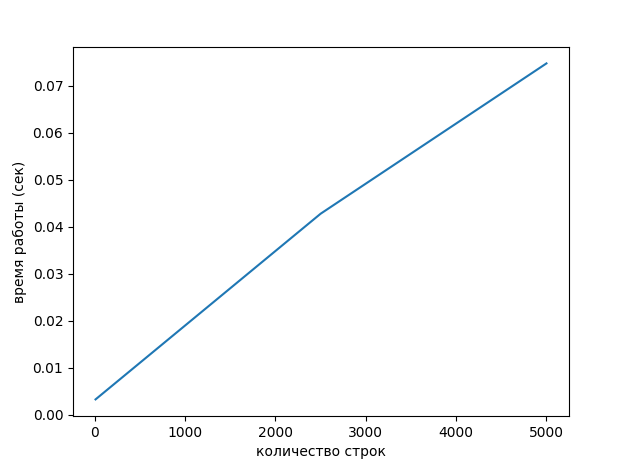
\includegraphics[width=\textwidth]{graph.png}
    \caption{График зависимости времени работы программы от количества запросов в файле}
\end{figure}


\subsection*{Точность}

Для оценки точности модели использовалась выборка данных из 5572 элементов, в которой каждому документу сопоставлялся тег спам/не спам.
В этой выборке предложения со спамом составляли 13\%.

\textbf{Precision}:  0.9726027397260274
\textbf{Recall}:  0.9594594594594594

% \newpage
\subsection*{Выводы}

В ходе курсового проекта я реализовал программу для классификации документов
с использованием наивного Байесовского классификатора.
Я узнал теоретические основы его работы и укрепил
навыки работы с текстовыми данными. 

В ходе выполнения проекта сложности возникали при правильной организации
структуры данных для классификации. Также была важной задача корректной работы
с вероятностями, особенно в случае редких слов в тексте.

Полученные навыки полезны для дальнейшей работы с текстовыми данными
и их обработкой, включая задачи анализа данных, создания систем рекомендаций
или автоматического распределения текстов по категориям, например, для определения спама.

\end{document}